\chapter{Vorgehen}
\label{ch_vorgehen} 
Das Ziel ist die Entwicklung eines Prototypen aus dem bestehenden Modell der Projektarbeit von \cite{PA_bicycle}. Die Vorgehensschritte sind in der untenstehenden Auflistung abgebildet. Sie bilden die Struktur dieses Kapitels. Die Definition der konkreten Schritte geschah in Absprache mit Prof. Dr. M. Meli und dem Resarch Assitenten Herr Dario Dünar vom Instiut of Embedded Systems (InES). Auf der CD finden sich die Sitzungsprotokolle über den aktuellen Entwicklungsstand, die offenen Fragen und die Entscheidungen.

\subsubsection*{Liste der Arbeitschritte}
\label{liste} 

\begin{enumerate}
  \item Inbetriebnahme Machbarkeitsstudie  
  \item Hardware entwickeln  
  \item Inbetriebnahme Prototyp      
  \item Energy und Power Management
  \item Entwickeln einer BLE-Applikation       
 \end{enumerate}  

Die sprachliche Unterscheidung von Energy - und Power Management entspricht der Unterscheidung zweier \glqq Management-Teilen\grqq im Prototypen: Das Endprodukt regelt an zwei Stellen auf unterschiedliche Art die zur Verfügung stehende Energie. Der Begriff Energy Management wird in dieser Arbeit für das Sammeln und Weiterleiten von Energie über eine Hardwareimplementation gebraucht. Der Begriff Power Management wird für die Softwareimplementation gebraucht. Diese regelt, dass die zur Verfügung gestellte Energie nicht sofort verbraucht wird. Die sprachliche Trennung ist künstlich, denn in der Umsetzung spielen Hard- und Softwareregelung Hand in Hand. Die sprachliche Unterscheidung dient der Lesbarkeit und bezeichnet keinen physikalischen Unterschied.
 
 
 % 1---------------------------------------------------------------------------
 %------------------------------------------------------------------------------
  
 
\section{Inbetriebnahme Machbarkeitsstudie}\label{v_inbetriebnahme} 

      
Ziel der Inbetriebnahme des Aufbaus der vorangehenden Arbeit \cite{PA_bicycle} ist es, zu definieren, welche Funktionalitäten verbessert werden sollen. Zur Orientierung werden im ersten Unterkapitel \ref{fb} die Funktionsblöcke und deren Aufgaben festgehalten. Danach wird das Verhalten der Vorgängermodells in Unterkapitel \ref{verhalten} ausgemessen. Aus der Analyse entsteht die in Unterkapitel \ref{optimierung} aufgelistete erste Optimierungsliste. Als letztes folgt eine Vertiefung in das auffällige Verhalten des Eingangssignals in Unterkapitel \ref{auffaellig}. Dieser Exkurs hat Ursache in der Begegnung mit  Ives Théoduloz von EM MicroElectronic. Er entwickelte den in dieser Arbeit verwendete EM8500-Chip mit und wies uns auf den auffälligen Signalverlauf des Harvester-Eingangssignals (siehe Abbildung \ref{spannungMachbarkeit}) hin. Dieses Signal wurde deshalb bei der Inbetriebnahme eigens getestet, was im letzten Unterkapitel dokumentiert ist.
      
\subsection{Funktionsblöcke}\label{fb} 

Der Bicycle Computer besteht aus vier Funktionsblöcken, die in der Abbildung \ref{funktionsdiagramm_bild} dargestellt sind. Der erste Funktionsblock ist der Harvester (siehe 1) in der Abbildung \ref{funktionsdiagramm_bild}). Die Aufgaben des Harvesters ist es Energie zu Ernten und dem nächsten Funktionsblock ( Nummer 2) in der Abbildung  \ref{funktionsdiagramm_bild} zur Verfügung zu stellen. Der zweite Funktionsblock wird als Energy Management-Teil in der Arbeit bezeichnet. Die Aufgabe des zweiten Blocks ist es, Energie zu Sammeln und kontrolliert an die Verbrauchsstelle freizuschalten. Detaillierte Informationen finden sich in den Theoretischen Grundlagen im Unterkapitel \ref{t_energy_management}. Der dritte Funktionsblock ist der Ort, an dem die Energie verbraucht wird. In dieser Arbeit dient die Energie dem Betreiben von Sensoren und dem versenden derer Daten. Dies wird auf dem Sensortag (siehe Anhang \ref{anhang_sensortag}) umgesetzt. Der Grund dafür wird in der Einleitung des Kapitels \label{t_power_management} dargelegt. Der letzte Funktionsblock bezeichnet das Ziel, das Erhalten von Sensordaten in einer Applikation.  

\begin{figure}[ht]
   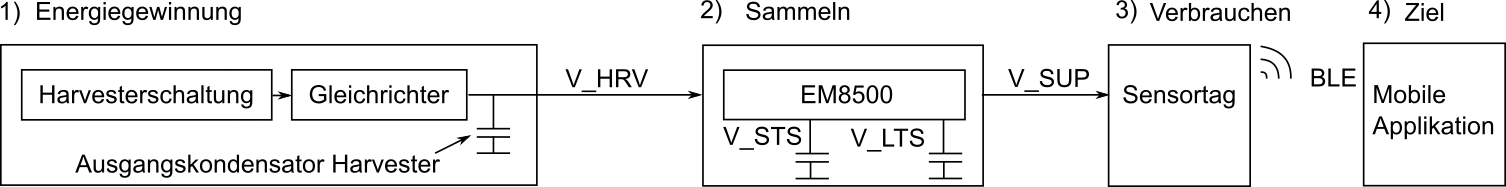
\includegraphics[width=1\textwidth]{3Vorgehen/imag/Blockdiagramm.png}
   \caption{Funktionsblöcke Bicycle Computer}
   \label{funktionsdiagramm_bild} 
\end{figure}

Den Funktionsblöcke sind Spannungsbezeichnungen sowie Kondensatoren beigefügt. Dies, weil bei der Beschreibung des Verhaltens des Vorgängermodells, diese Spannungslevel für die Funktionsbeurteilung wichtig werden. Die nachfolgende Legende beschreibt die Beschriftung näher.

\subsubsection*{Legende Abbildung \ref{funktionsdiagramm_bild} }
\label{legende}
\begin{tabbing}
    Bezeichnung \quad\= Beschreibung\\[0.8ex]
    V\_HRV \> Ausgangspannung Harvesterquelle, Eingangsspannung Energy Management\\
    V\_STS\> Spannung am STS--Kondensator (Primärspeicher)\\
    V\_LTS\> Spannung am LTS--Kondensator (Sekundärspeicher)\\
    V\_SUP\> Ausgangsspannung Energy Managment, Eingangsspannung Sensortag\\
    BLE \> Senden der Daten per Bluetooth Low Energy (siehe \ref{t_ble} \\
\end{tabbing}   

\todo{Header Tabelle (Bezeichnung, Beschreibung) weg } 

\subsection{Verhalten des Vorgängermodells}\label{verhalten} 

Die Inbetriebnahme bestätigte das in der Dokumentation \cite{PA_bicycle} beschriebene Verhalten. Die Abbildung \ref{spannungMachbarkeit} zeigt den zeitlichen Verlauf der Energiestände zwischen den Funktionsblöcken (siehe Abbildung \ref{funktionsdiagramm_bild} und an den Speicherelementen. Die Legende zur Abbildung  \ref{spannungMachbarkeit} erklärt die Signale.

\begin{figure}[ht]
    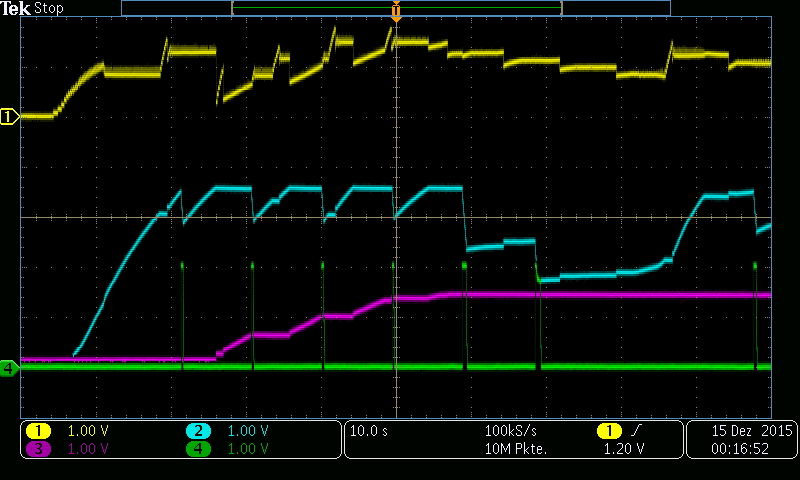
\includegraphics[width=0.5\textwidth]{3Vorgehen/imag/messungPA.png}
    \caption{Spannungswerte Modell der Machbarkeitsstudie}\label{spannungMachbarkeit} 
\end{figure}

\subsubsection*{Legende Abbildung \ref{spannungMachbarkeit} }
\begin{tabbing}
    Channel\quad\= Farbe\quad\= Beschreibung\\[0.8ex]
    CH1\> gelb\> Spannungsverlauf V\_HRV\\
    CH2\> blau\> Spannungsverlauf am STS--Kondensator\\
    CH3\> violet\> Spannungsverlauf am LTS--Kondensator\\
    CH4\> grün\> Ausgangsspannung nach Energy Management\\
     \>  \>      Eingangsspannung Sensorttag
\end{tabbing}    

Im Folgenden werden die einzelnen Spannungsverläufe chronologisch der Kanalnummer nach analysiert. Kanal 1 spiegelt die Spannung am Harvesterausgang wieder (V\_HRV). Gemäss Theorie \ref{eingangsspannung} bzw. gemäss Datenblatt des EM8500 ist der EM8500-Chip für ein DC-Signal ausgelegt. Er geht von einem regelmässigen Eingangssignal aus und regelt die Spannung auf den MPPT. Diese Regelung sollte wie in Abbildung \ref{RegelungSpannung} aussehen. Das reale Signal entspricht nicht diesem Verhalten. Die Regelung ist abrupt und überspringt mehrere Spannungslevel. Der Ursache für die schlechte Regelung soll nachgegangen werden.

Kanal 2, blau, gibt den Spannungsverlauf am Hauptspeicher, dem Primärspeicher, der in der im Datenblatt von EM8500 STS heisst, wieder. Das Energy Management des Vorgängermodells setzt den Schwellwert für den Primärspeicher (STS) mit 3.6 V hoch (Details zu den Schwellwerten im Kapitel Theoretische Grundlagen \ref{t_energy_management}). Der hohe Wert erklärt durch das Ziel, genug Energie für ein konstantes Paketversenden zu haben. Dies gelingt für fünf BLE-Pakete. Danach reicht die Energie nicht mehr aus. V\_SUP, grünes Signal, wird nicht mehr gespiesen. Nach 30 s ohne Pakete senden ist wieder genug Energie gespeichert, für weitere 5 Datenpakete.

In der Auswertung viel uns auf, dass dieser Signalverlauf nur bei einer Geschwindigkeit 45 km/h möglich ist. Die Speicherkapazität von 470 $\mu$F und ein Schwellwert der Spannung von 3.6 V ist mit normaler Geschwindigkeit (10 km/h) nach 30 min nicht zu erreichen. Fährt man rund 45 km/h so erhält man die in der Abbildung gezeigte Ladezeit von rund 25 s. Eine exakte Geschwindigkeitsmessung ist zu Beginn der Arbeit nicht möglich. Das Rad wird von Hand gedreht und mit einem Metronom wird die Umdrehungsgeschwindigkeit vorgegeben. Bei einem Radumfang von 2.04 m und einer Zeitdifferenz von 160 ms zwischen den Reed-Inpulsen, ergibt die Geschwindigkeit von 45 km/h. Da diese Messmethode über längere Zeit nicht sehr genau ist, bestand eine der Aufgabe nach der Inbetriebnahme im Organisieren eines Messaufbaus. Dieser professionellere Messaufbau wird im Anhang \ref{messaufbau} beschrieben.


Kanal 3, das pinkige Signal, zeigt die Spannung am Long Time Speicher. Die Inbetriebnahme zeigt, dass sich der LTS lädt. Es erstaunt jedoch, dass seine geerntete Energie nicht verwendet wird. Der Spannungswert von LTS geht nie herunter.
Die Vermutung ist, dass der eingestellte Schwellwert für den Bezug von Energie von LTS \ref{energiespeisung_lts} nicht stimmt.

Kanal 4, das grüne Signal, zeigt, die Speisung des Sensortags. In Modell der Projektarbeit steuert der Microkontroller des Sensortags den Verbraucht. Alle 10 s wacht das System auf, bezieht Energie vom EM8500-Ausgang für das Senden eines Paketes und geht dann wieder schlafen. Das Aufwachintervall ist fix.


\subsection{Optimierungsliste}\label{optimierung} 

\todo{ Ev. Texbausteine von oben hier hin}

Aus den Messungen der Inbetriebnahme konkretisierten sich die generellen Aufgaben, die in der ersten Liste der Arbeitsschritte zu Beginn des Vorgehens  beschrieben wurden. Folgende vier Punkte sollen durch den Prototypen verbessert werden: 

\begin{itemize}
     \item Der Verlauf des Harvester-Eingangs wechselt abrupt. Der Eingang soll besser geregelt werden. 
     \item Das Laden des Primärspeichers von 470 $\mu$F in 25 s benötigt es eine Geschwindigkeit von mehr als 60 km/h.  Die Harvesterschaltung soll so weiterentwickelt werden, dass bei 10 km/h genug Energie zum Senden von BLE-Paketen besteht.    
     \item Das zweite Speicherelement, der LTS, entlädt sich nicht. Dadurch kann seine Energie nicht verwendet werden. Die Schwellwerte am EM8500 und ev. die Kondensatorenwerte sollen so angepasst werden, dass sich der zweite Kondensator entlädt
     \item Die Energie wird statisch nach einem fixen Zeitintervall von 10 s genutzt. Das Zeitintervall soll der Geschwindigkeit angepasst werden. Bei höherer Geschwindigkeit soll das Intervall kürzer werden.
\end{itemize} 


Im Resultatsteil Kapitel \ref{ch_resultat} werden die Fortschritte in diesen vier Punkten ausgewiesen.

\subsection{Vertiefung in auffälliges Verhalten des Harvestereingangs}\label{auffaellig} 


Text aus Einleitung: Für Argumentation. (Als letztes folgt eine Vertiefung in das auffällige Verhalten des Eingangssignals in Unterkapitel \ref{auffaellig}. Dieser Exkurs hat Ursache in der Begegnung mit  Ives Théoduloz von EM MicroElectronic. Er entwickelte den in dieser Arbeit verwendete EM8500-Chip mit und wies uns auf den auffälligen Signalverlauf des Harvester-Eingangssingals (siehe Abbildung \ref{spannungMachbarkeit}) hin. Dieses Signal wurde deshalb bei der Inbetriebnahme eigens getestet, was im 

??????  .... folgte.) Hier ist nun dieser erwähnte Text.

Vorschlag Katrin:
Die auffällige Regelung des Harvesterinputs wurd Ives Théoduloz gezeigt. 

Gemäss Ives Théoduloz sollten Kondensatoren der Harvesterschaltung im Bereich von 4.7 $\mu$F liegen, sodass die Energiemanagementschaltung ordnungsgemäss funktioniert.  


In der Machbarkeitsstudie ist nach dem Gleichrichter ein Kondensator von 470 $\mu$F nachgeschaltet. Dieser glättet die Spannungspulse nach dem Gleichrichter zu einer DC-ähnlichen Spannung mit Rippeln.

Aus diesem Grund wird die Rippelspannung am Ausgangs der Harvesterschaltung mit kleineren Kondensatoren gemessen. Das Messprotokoll befindet sich im Anhang.

\subsubsection{Ausmessen der Auswirkung des Ausgangskondensators}
\todo{auf Messprotokoll verweisen}

Mit einem Kondensator von 470 $\mu$F wird die Ausgangsspannung der Harvesterspannung fast rippelfrei. Die Rippelspannung beträgt 3.2 mV (siehe Abbildung \ref{kond470uF}).

\begin{figure}
    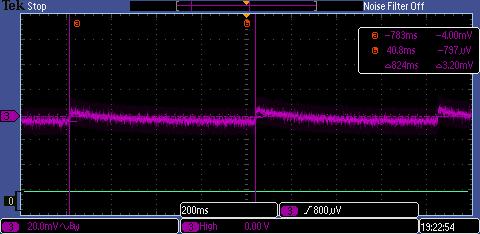
\includegraphics[width=15cm]{3Vorgehen/imag/470uF.PNG}
    \caption{Rippelspannung bei Glättung mit 470 $\mu$F Kondensator}\label{kond470uF} 
\end{figure}

\subsubsection*{Messaufbau}
In der gegebenen Harvesterschaltung wird am Kondensator die Spannung mit einem Kathodenstrahloszilloskop (KO) gemesssen. Ausgehend vom bestehenden Kondensator (470 $ \mu $F), werden danach Elektrolytkondensatoren (Elko) mit den Werten 100 $\mu F $F, 47 $\mu$F und 10 $\mu$F gemessen.

\begin{figure}[h]
    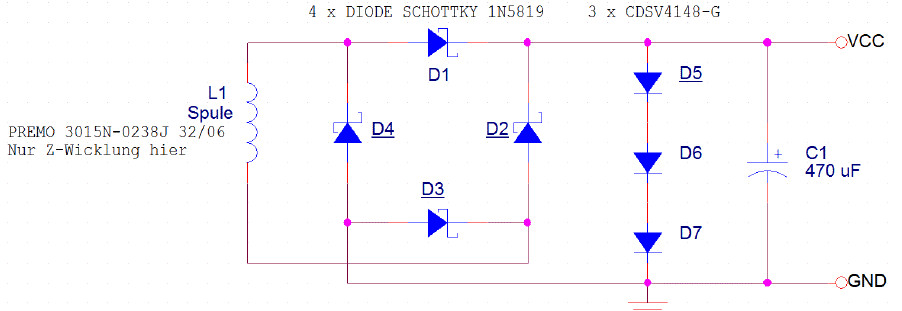
\includegraphics[width=15cm]{3Vorgehen/imag/messschaltungHarvesterschaltung.jpg}
    \caption{Messschaltung}
\end{figure}

\subsubsection*{Resultat}

Die Rippelspannung erhöht sich wie erwartet. Vpp beträgt bei 100 uF \textbf{xx} mV, bei 47 uF 28.8 mV (siehe Abbildung \ref{kond47uF}) und bei 10 uF 320 mV (Abbildung \ref{kond10uF}).
 
\begin{figure}
    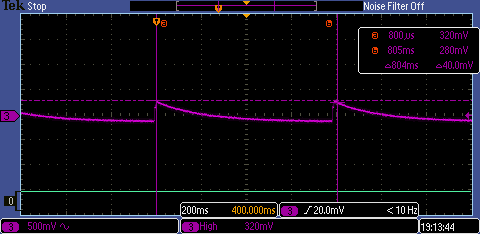
\includegraphics[width=15cm]{3Vorgehen/imag/10uF.PNG}
    \caption{Rippelspannung mit 10 uF Kondensator}\label{kond10uF} 
\end{figure}

\begin{figure}
    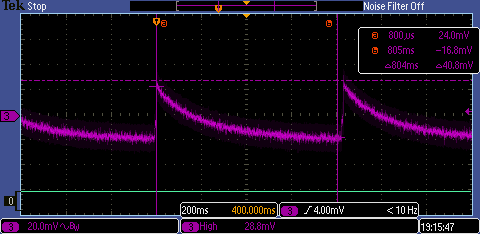
\includegraphics[width=15cm]{3Vorgehen/imag/47uF.PNG}
    \caption{Rippelspannung mit 47 uFKondensator}\label{kond47uF} 
\end{figure}

Nach Rücksprache mit einem Entwickler des EM8500-Chips wird der zu hohe Kondensator vor dem Harvester-Eingang als Ursache vermutet. Laut Datenblatt sollte dieser 4.7 $\mu$F, damit der Booster mit eingebautem MPPT ideal regeln kann.


Aus den Beobachtungen ergaben sich folgende Aufgaben für die Entwicklung des Prototypen:

\begin{enumerate}
    \item Die Harvesterschaltung funktioniert nicht optimal. Die Auswirkung des zu hohen Kondensator vor Harvestereingang soll getestet werden
    \item Die Schaltung soll für eine Geschwindigkeit von 10 km/h ausgelegt werden
    \item Die Konfigurationen beim EM8500 sollen überarbeitet werden, sodass LTS genutzt wird
    \item Das Senden der Pakte soll der Geschwindigkeit angepasst werden
\end{enumerate}

Punkte 1 und 2 haben Auswirkung auf das Layout, Punkte 3 und 4 auf die 





%------------------------------------------------------------------------------
% 2---------------------------------------------------------------------------
%------------------------------------------------------------------------------



\section{Hardware entwickeln}
Aus der Inbetriebnahme der Machbarkeitsstudie, wurden einige Punkte ersichtlich, welche mit einer neuen Leiterplatte, bzw. einer neuen Hardware verbessert werden können. Im speziellen muss die Harvesterschaltung genauer angeschaut werden und es soll versucht werden die nachfolgenden Punkte aus der Inbetriebnahme der Machbarkeitsstudie umzusetzen. 

-	Die Schaltung soll für eine Geschwindigkeit von 10 km/h ausgelegt werden

Ausserdem soll die neue Leiterplatte den fliegenden Aufbau der Harvesterschaltung und den EM-Chip beherbergen. Es wird in diesem Schritt darauf verzichtet, das TI-SensorTag ebenfalls in die neue Leiterplatte zu integrieren, da die Komplexität des TI-SensorTags hoch ist und die Hardware gut in mehreren Schritten überarbeitet werden kann.
\subsection{Schema}
Bevor ein Leiterplattenlayout entwickelt werden kann, muss das Schema erfasst werden. Es wurden verschiedenste Vorgaben von den Dozenten vorgegeben, welche im besten Fall alle eingehalten werden. Die Grösse der Leiterplatte soll die Grösse des TI-SensorTags nicht überschreiten, alle Netze sollen mit Testpunkten ausgestattet werden, alle Anschlüsse des TI-SensorTags auf der Leiterplatte zugänglich sein und alle Testpunkte des TI-SensorTags sollen im Rastermass 2.5 mm angeordnet werden. Ausserdem sollten, falls der Platz ausreichen würde, Strommesspunkte an der Speisung des TI-SensorTags, des Longterm Storage und des Shortterm-Storage angebracht werden. Diese Vorgaben sollen die Leiterplatte für eventuelle Laborübungen der Schule verwendbar machen. Das Schema besteht im groben aus vier Teilen:
\begin{enumerate}
    \item Harvesterschaltung
    \item EM-Chip inklusive zugehöriger Peripherie
    \item Energiespeicher
    \item Umlauferfassung
\end{enumerate}

\subsubsection{Harvesterschaltung}
Die Harvesterschaltung wurde in der Machbarkeitsstudie als fliegender Aufbau realisiert, was zu einigen Problemen führen kann, da viele lange Kabel verwendet wurden und somit die Signallaufwege ziemlich lang sind. Bisher hat dies keine Probleme verursacht, doch es geht wichtige Energie in den Kabeln verloren. Ebenfalls wurde in der Inbetriebnahme bemerkt, dass die gewonnene Leistung sehr gering ist, weswegen die Schaltung in einem zweiten Schritt optimiert werden muss.
\begin{figure}
    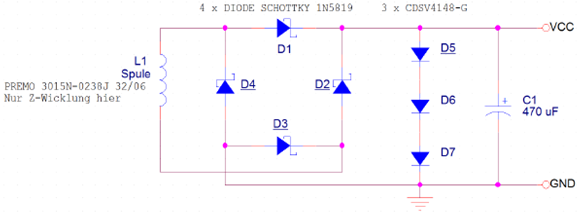
\includegraphics{3Vorgehen/imag/Schema_Harvester_PA.PNG}
    \caption{Harvesterschaltung der PA15}\label{schema_harvester_pa15} 
\end{figure}
Die Harvesterschaltung der Abbildung ref{schema_harvester_pa15}} wurde im Rahmen der Machbarkeitsstudie erarbeitet. Die Schaltung besteht aus wenigen Teilen, die Spannungbegrenzung wurde mit drei Dioden in Durchlassrichtung realisiert, hier gibt es wahrscheinlich bessere Möglichkeiten die Spannung zu begrenzen, ohne unnötig Leistung zu verschwenden.
\subsubsection{EM-Chip}
Das EM-Evaluationsboard soll ebenfalls auf der neuen Leiterplatte Platz finden, das Schema inklusive aller Kondensatoren ist im Datenblatt zu finden. Jedoch wurden die Jumper nicht übernommen und nur einige Stecker wurden übernommen, bzw. mit eigenen Signalen ergänzt.
\begin{figure}
    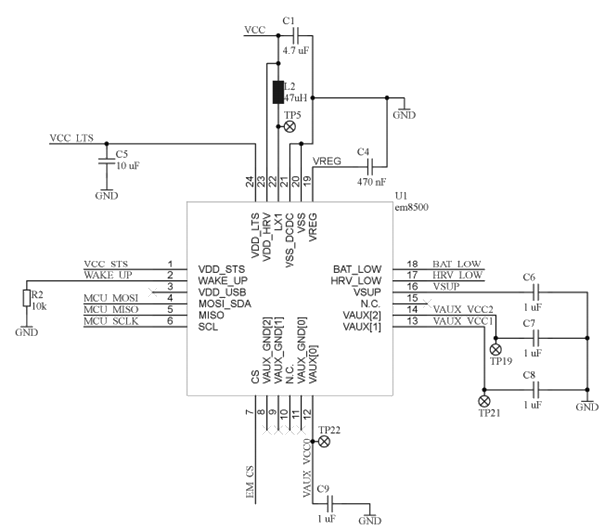
\includegraphics{3Vorgehen/imag/Schema_EM-Chip_inkl_Peripherie.PNG}
    \caption{Schema des EM-Chips mit der benötigten Peripherie}\label{schema_em-chip_inkl_peripherie} 
\end{figure}

\subsubsection{Energiespeicher}
Die Energiespeicher sollten flexibel gestaltet werden, da die genaue Art, bzw. Dimensionierung noch nicht definitiv war und noch Tests bezüglich der Energiespeicher anstanden. Jedoch wurde im Schema jeweils ein Elko als Platzhalter verwendet, da in der Machbarkeitsstudie ebenfalls Elkos verwendet wurden, die Kapazitätswerte sind jedoch nur erste Werte, welche nur abgeschätzt wurden.
\begin{figure}
    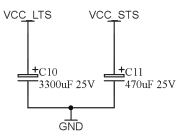
\includegraphics{3Vorgehen/imag/Schema_Energiespeicher.PNG}
    \caption{Schema der Energiespeicher (Elkos sind nur Platzhalter)}\label{schema_energiespeicher} 
\end{figure}

\subsubsection{Umlauferfassung}
Die Umlauferfassung kann nicht mit der verwendeten Spule realisiert werden, da die Energie aus der Spule gewonnen wird. Die nicht benutzten Wicklungen der X- und Y-Wicklung liefern kein klares Signal, was bereits in der Machbarkeitsstudie bewiesen wurde. Aus diesem Grund wird der Magnetdurchlauf mit einem Reedswitch detektiert und an das TI-SensorTag weitergegeben. Ein Magnetdurchlauf erzeugt einen positiven Puls, solange der Magnet in der Reichweite des Reedswitch befindet.
\begin{figure}
    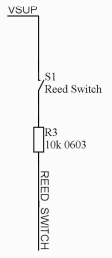
\includegraphics{3Vorgehen/imag/Schema_Umlaufdetektion.PNG}
    \caption{Schema Umlauferfassung}\label{schema_umlaufdetektion} 
\end{figure}

\subsection{Bauteildefinition und Optimierung}
Nachdem klar war, welche Teile auf der Leiterplatte Platzfinden müssen, konnte die Optimierung der Schaltung in Angriff genommen werden. Ziel der Optimierung war es bei 10 km/h genügend Energie zu gewinnen, damit das TI-SensorTag damit versorgt werden könnte. Dafür musste vorallem die Harvesterschaltung optimiert werden, damit keine Energie unnötig verloren geht. 
Es wurden folgende Punkte angeschaut und versucht zu optimieren:
\begin{enumerate}
    \item die Spule
    \item der Gleichrichter
    \item der Limiter
\end{enumerate}
\subsubsection{Die Spule}
Die Spule gewinnt die Energie aus dem an einer Speiche des Fahrrads befestigten Magneten. Eine bessere Spule könnte mehr Energie aus dem vorbei schnellenden Magneten gewinnen. Entscheidend ist das die Fläche der Spule nicht vergrössert werden darf, bestenfalls sollte eine kleinere Spule gefunden werden, welche mehr Energie gewinnt. Gemäss der Formel 2.4 ist für die gewonnene Energie vor allem die Wicklungszahl entscheidend, jedoch wird bei den Spulen meistens nur die Induktivität angegeben. Dies ist kein Problem, da die Induktivität quadratisch von der Wicklungszahl (siehe Formel x) abhängt.
\todo{Formel einfügen (Referenz: https://home.zhaw.ch/~spma/Scripts/ET_ST/EL2/Theorie/Induktivitaet.pdf (Konsultierung am 02.06.16))}
Es wurde nach einer Spule mit einer höheren Induktivität und der gleichen Fläche gesucht, somit können nur noch zwei Variablen sich verändern. Zum einen kann sich die Wicklungszahl verändern und zum andern kann sich die Länge der Spule verändern. Die Spule von Würth Elektronik hat eine ähnliche Fläche und eine grössere Induktivität, was auf den ersten Blick sehr vielversprechend aussieht.

Die Messung der erzeugten Spannung über der Spule hat ergeben, dass die Spule von Premo, welche bisher verwendet wurde, eine höhere Spannung erzeugt als die neue Spule von Würth. Die Spule von Premo mit der Bezeichnung 3015N 0238J 3206 hat bei den Geschwindigkeiten von 10 km/h und 20 km/h eine grössere induzierte Spannung. Die Spule von Würth mit der Bezeichnung 74458308 hat eine höhere Spannung bei den Geschwindigkeiten von 15 km/h und 40 km/h. Jedoch sollte die Schaltung für 10 km/h optimiert werden, somit muss der Spule von Premo der Vortritt gerwährt werden. Nachfolgend wird der Unterschied zwischen den induzierten Spannungen in den Spulen ersichtlich (siehe Abbildung \ref{messung_optimierung_spule}. Der Unterschied ist nicht gross, jedoch muss hier die Spule von Premo bevorzugt werden, da die induzierte Spannung grösser ist.
\begin{figure}
    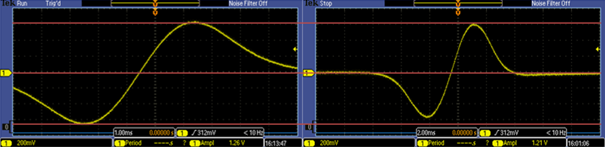
\includegraphics{3Vorgehen/imag/Messung_Optimierung_Spule.PNG}
    \caption{Links: Spannung über der Spule von Premo, Rechts: Spannung über der Spule von Würth, Geschwindigkeit 20 km/h}\label{messung_optimierung_spule} 
\end{figure}

\subsubsection{Der Gleichrichter}
Der Gleichrichter aus der Machbarkeitsstudie bestand aus vier Dioden vom Typ 1N5819. Diese Dioden sind nicht für die LowPower-Anwendung ausgelegt, ausserdem sind die Dioden nicht ein einem Gehäuse verbaut. Wichtig ist bei dem Gleichrichter, dass die Leckströme möglichst klein sind und die Schwellenspannung sollte ebenfalls möglichst klein sein.

Es wurde als erstes eine LowPower-Diode, mit der Bezeichnung HSMS-286P, getestet, die Erwartungen waren entsprechend hoch, da diese Dioden für LowPower-Anwendungen spezialisiert ist. Die Spule von Premo wurde als Quelle verwendet, um zu sehen, wie die Spannung nach dem Gleichrichter aussieht. Die Spannung nach dem Gleichrichter bestehend aus den Dioden vom Typ 1N5819 ist bei allen getesteten Geschwindigkeiten, also 10 km/h, 15 km/h, 20 km/h und 40 km/h, höher als beim Gleichrichter bestehend aus den Dioden vom Typ HSMS-286P. Der Spannungsunterschied liegt im Minimum bei ca. 40mV. Der grösste Unterschied ist bei der Geschwindigkeit von 15 km/h ersichtlich, was in der Abbildung \ref{messung_optimierung_gleichrichter_1} gezeigt wird.
\begin{figure}
    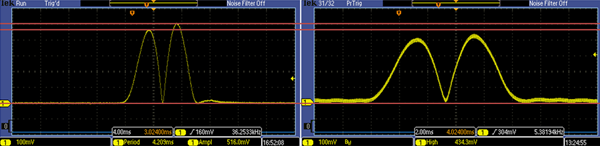
\includegraphics{3Vorgehen/imag/Messung_Optimierung_Gleichrichter_1.PNG}
    \caption{Links: Gleichrichter 1N5819, Rechts: Gleichrichter aus HSMS-286P, 15 km/h}\label{messung_optimierung_gleichrichter_1} 
\end{figure}
Als nächstes wurde ein Gleichrichter aus den Dioden vom Typ BAT54 getestet. Die Spannung nach dem Gleichrichter bestehend aus 1N5819 Dioden ist bei den Geschwindigkeiten von 15 km/h, 20 km/h und 40 km/h höher als nach dem Gleichrichter bestehend aus BAT54 Dioden. Der Spannungsunterschied liegt bei ca. 100 mVpp, der Unterschied ist marginal, jedoch muss hier der Gleichrichter aus 1N5819 Dioden bevorzugt werden. Nur bei einer Geschwindigkeit von 10 km/h ist der Gleichrichter bestehend aus BAT54 Dioden besser als der Gleichrichter bestehend aus 1N5919 Dioden. Der Spannungsunterschied liegt hier bei ca. 10mVpp, dieser Unterschied ist vernachlässigbar, in Angesicht, dass der Gleichrichter bestehend aus 1N5819 Dioden in allen anderen getesteten Geschwindigkeiten besser ist.
\begin{figure}
    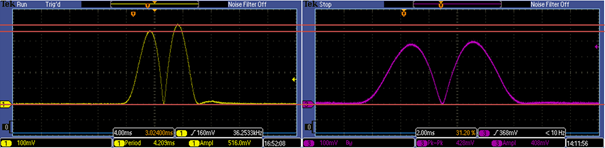
\includegraphics{3Vorgehen/imag/Messung_Optimierung_Gleichrichter_2.PNG}
    \caption{Links: Gleichrichter 1N5819, Rechts: Gleichrichter aus BAT54, 15 km/h}\label{messung_optimierung_gleichrichter_2} 
\end{figure}

\subsubsection{Der Limiter}
Die Spannungsbegrenzung, nachfolgend der Limiter genannt, ist ein sehr krititscher Teil der Harvesterschaltung, da die Spannung am EM-Chip Eingang nicht höher als 2V sein darf, da ansonsten der EM-Chip beschädigt werden kann. Trotzdem soll möglichst wenig Energie verloren gehen, wenn die Spannungsbegrenzungsschaltung ihre Arbeit verrichtet. Bisher wurden drei Dioden in Durchlassrichtung in Serie geschalten, um die Spannung zu begrenzen.

Herr Erich Ruff hat eine Spannungsbegrenzungsschaltung entwickelt, welche er uns freundlicherweise zur Verfügung stellte. Diese Schaltung wurde mit dem Limiter verglichen, welcher aus drei Dioden bestand.

Die Spannung nach dem Dioden-Limiter ist bei 10 km/h, 15 km/h und 20 km/h höher, jedoch ist die Rippelspannung ebenfalls höher. Nur bei einer Geschwindigkeit von 40 km/h ist die Spannung nach dem LImiter von Herr Erich Ruff, nachfolgend FET-Limiter genannt, besser sowohl bei Spannungslevel als auch bei der Rippelspannung. Die Abbildung x zeigt, dass der Dioden-Limiter eine höhere Spannung liefert, jedoch ist die Rippelspannung ebenfalls höher.
\begin{figure}
    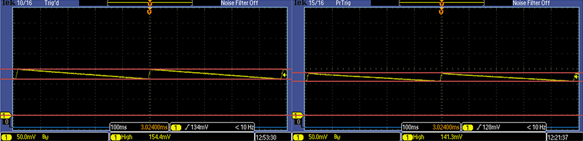
\includegraphics{3Vorgehen/imag/Messung_Optimierung_Limiter.PNG}
    \caption{Links: Dioden-Limiter, Rechts: FET-Limiter, 15 km/h}\label{messung_optimierung_limiter} 
\end{figure}

\subsection{Layout}
Schlussendlich musste aus den optimierten Teilen des Schemas eine Leiterplatte gestaltet werden. Die meisten Footprints waren bereits in den Bibliotheken des IneS vorhanden, einige mussten neu gezeichnet werden.
\subsubsection{Positionierung}
Die Positionierung der einzelnen Teile kann sehr wichtig sein, da mit einer guten Positionierung bereits unnötige Leiterbahnverläufe verhindert werden können. Ebenfalls können gut positionierte Bauteile die Spannungspegel stabilisieren. Es wurde darauf geachtet die Bauteile, welche zu einem Block gehören, nahe beieinander platziert wurden, um unnötig lange Signallaufwege zu verhindern.

Die Bauteile der Harvesterschaltung wurde als Block so nahe wie möglich beieinander platziert und wo immer möglich wurden die Speisungsleitungen mit 20 Mil gezogen, damit der Widerstand der Leiterbahn möglichst klein gehalten wurde. Der Leiterwiderstand konnte so minimiert werden, was verhindert, dass die Energie in den Leiterbahnen verschwendet wird.
\todo{Formel für Leiterwiderstand einfügen}
Der Widerstand bei 10 Mil ist somit 2.4 mΩ, der Leiterwiderstand bei einer Leiterbahnbreite von 20 Mil ist 1.2 mΩ. Problematisch ist, dass der Block der Harvesterschaltung etwas entfernt vom Block des EM-Chips befindet, das bedeutet, die Leiterbahn mit der Speisung des EM-Chips muss mehrere Zentimeter zurücklegen. Sicherlich ist der Unterschied im Widerstand nicht sehr gross, doch die Energie, welche in der Leiterbahn verloren gehen würde, konnte so halbiert werden.

Der wichtigste Aspekt der Platzierung des EM-Chips war, dass die Stützkondensatoren so nah wie möglich am EM-Chip platziert wurden, damit die Spannung am EM-Chip so konstant wie irgend möglich gehalten werden kann.

Ein weiterer wichtiger Punkt war die Platzierung des Steckers, welcher unsere Leiterplatte mit dem TI-SensorTag verbindet, durch eine Falschplatzierung kann es hier passieren, dass die beiden Leiterplatten nicht schön übereinander sind, wenn sie aufeinander gesteckt werden. Das ist eher ein ästhetisches Problem, jedoch kann das auch Problem beim Einbauen in ein eventuelles Gehäuse bereiten. Zu dem Stecker gehört auch die Paltzierung der Testpunkte, welche direkt mit dem Stecker verbunden sind. Gemäss dem Wunsch der Betreuer wurde hier ein Rastermass von 2.5mm der Testpunkte eingehalten, so dass eine Steckerleiste eingelötet werden könnte. Problematisch ist jedoch, dass die Testpunkte einen grossen Raum der Leiterplatte einnehmen, wie in Abbildung \ref{layout_testpunkteraster}} ersichtlich.
\begin{figure}
    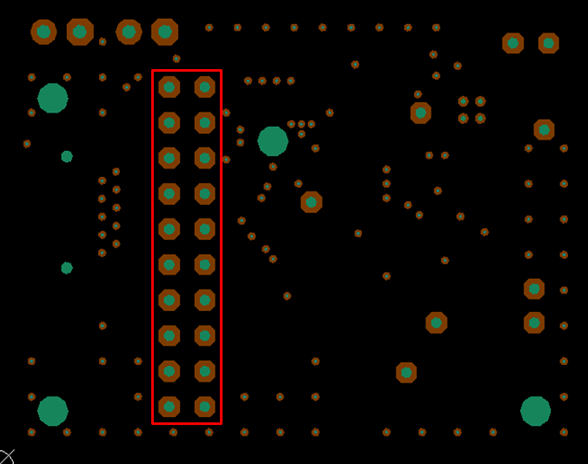
\includegraphics{3Vorgehen/imag/Layout_Testpunkteraster.PNG}
    \caption{Pads der Leiterplatte, rot eingerahmt die Testpunkte des Steckers}\label{layout_testpunkteraster} 
\end{figure}

\subsubsection{Das erste Layout}
Die erste Version der Leiterplatte war mit vielen Wünschen der Betreuer ausgestattet. Alle Netze wurden mit Testpunkten ausgestattet, die Testpunkte des Steckers wurden im Rastermass 2.5mm angeordnet und die Netze der Spannung nach dem Harvester, die Spannung des Short- und Long-Term-Storage wurden mit Strommesspunkten ausgestattet. Es wurden ebenfalls Montagelöcher platziert, jedoch sind diese sehr minimalistisch, da nur eine M2-Schraube durch passt, besser wäre es Montagelöcher für M3-Schrauben zu platzieren, doch der Platz auf der Leiterplatte ist sehr limitiert. Die Leiterplatte ist nur 33x42mm gross, was ein Milimeter breiter ist, als das TI-SensorTag. Der Anschluss der Energiespeicher wurde so realisiert, dass die Energiespeicher nicht auf der Leiterplatte Platz finden, sondern über ein Kabel oder Litze mit der Leiterplatte verbunden werden können.

\subsubsection{Das Redesign}
Ein grosser Fehler wurde in der Umsetzung des Steckers begangen, denn sowohl die Platzierung als auch der Footprint wurden falsch umgesetzt. Der Stecker wurde nicht an der richtigen Stelle platziert, somit überlappte unsere Leiterplatte das TI-SensorTag. Beim Erstellen des Footprints des Steckers wurden die Pins vertauscht, dort wo der Pin 1 sein sollte wurde der Pin 19 platziert und umgekehrt. Dies musste korrigiert werden, damit unsere Leiterplatte direkt mit dem TI-SensorTag verbunden werden kann. Dafür wurde die Leiterplatte überarbeitet, jedoch war die Zeit zu knapp, als dass die Leiterplatte für Tests vorhanden war.
\begin{figure}
    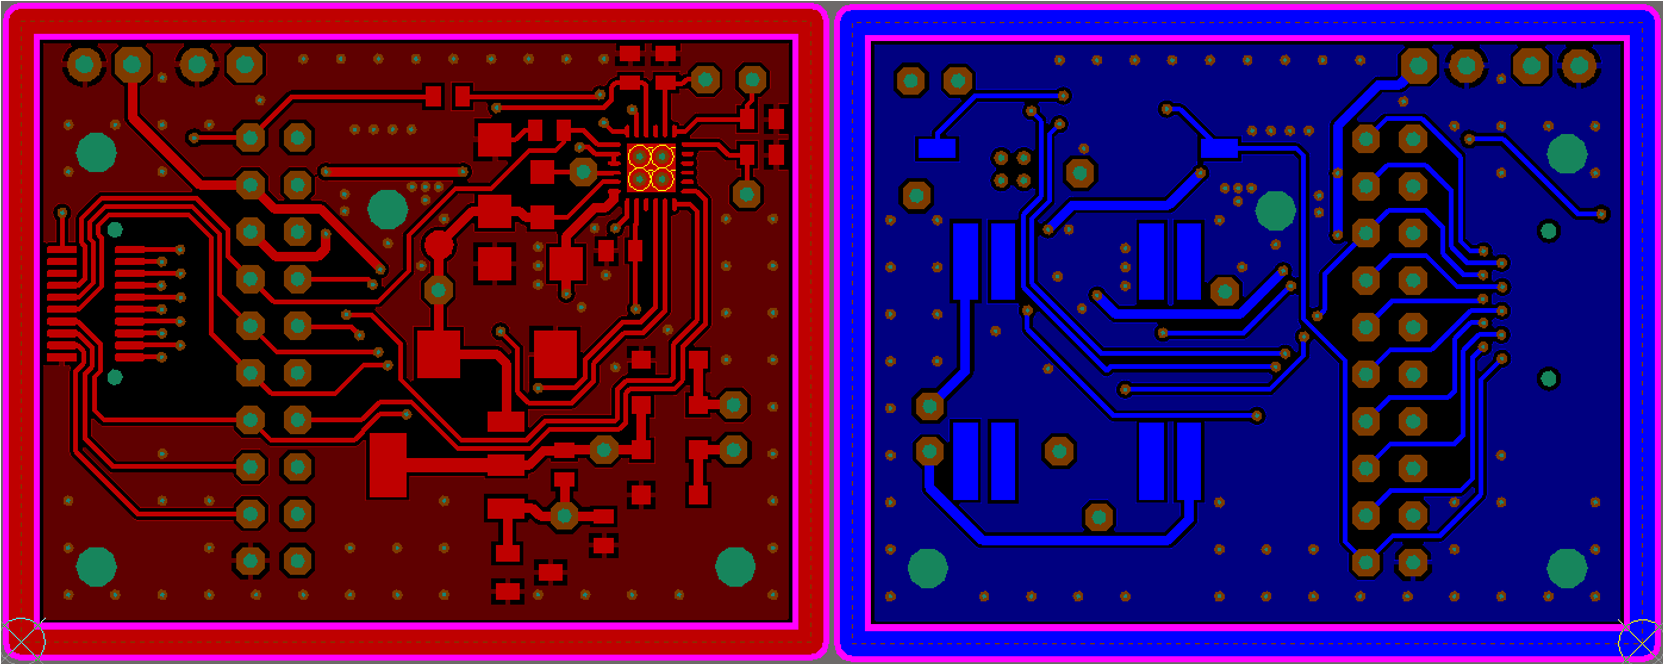
\includegraphics{3Vorgehen/imag/Layout_Redesign.PNG}
    \caption{Links: Top-Layer, Rechts: Bottom-Layer}\label{layout_redesign} 
\end{figure}

\todo{ Namensklärung: V HRV = VCC}
\todo{Messprotokolle umbenennen}

% 4----------------------------------------------------------
\section{Inbetriebnahme des Prototypen}
Ziel des Kapitels: Ausmessen und sehen, dass zu wenig Energie. (Weglassen. Testteil). 2. Magnete nach 180 \% (Bild), Reellight bringt idee für 2 Magnete hintereinander, besser Spule verwenden

--- alter Text
Der entwickelte Prototyp wurde intensiv ausgemessen (siehe Messprotokolle XXXX.)  Es werden 3 Messstellen unterschieden siehe Abbildung \ref{EnergieMessungStellen}. In den folgenden Unterkapiteln werden die Resultate und die darauf folgenden Entwicklungsschritte kurz beschrieben:

\begin{figure}
  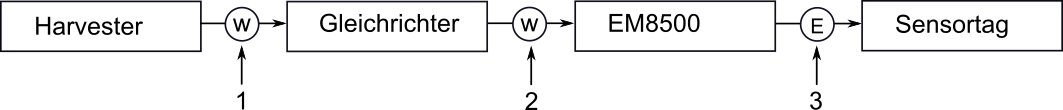
\includegraphics[width=1.0\textwidth]{3Vorgehen/imag/EnergiemessungStellen.png}\label{EnergieMessungStellen} 
  \caption{Messstellen am Prototypen}
\end{figure}

\subsection{Testen der Harvesterschaltung}

- Zu wenig Energie
- Zwei Magnete
- stärkere Spule

\subsection{Ausmessen der Energie vor und nach dem Gleichrichter}


\subsection{Energiemessungen nach dem EMBoard}



% 5---------------------------------------------------------------------------
\section{Energy Management}

Die Primäraufgabe des Energy Managements ist es, dass die zur Verfügung stehende Energie bei 10 km/h genügt, zum BLE-Pakete zu versenden. Die sekundäre Aufgabe ist es, dass man erreicht, dass sich der Long Time Storage entweder nicht lädt oder aber sich auch entlädt. Ein Laden des LTS ohne Energieabgabe ist Energieverschwendung. Die zwei gestellten Aufgaben sollen durch möglichst optimale Speichergrössen und intelligente Schwellwerte erreicht werden.

Damit man die Kondensatorenwerte berechnen kann, braucht es Energiedaten. Deshalb stehen im ersten Unterkapitel \ref{v_messungen_sensortag} Messergebnisse, danach folgt im zweiten Unterkapitel \ref{v_e_kalkulation} die Dimensionierung der Kondensatoren und dann das Berechnen der Schwellwerte in Unterkapitel \ref{v_schwellwerte}. Als letzer Punkt werden aufgrund der Ladewerte der Kondensatoren Energiezustände definiert. Dies, weil die letzte offene Aufgabe der Optimierunsliste \ref{optimierung}: Das Ersetzen des fixen Paketversendens nach 10 s dem Energiezustand angepasst werden soll. Die Vorgehensweise zur Erfüllung dieses Punktes ist im letzten Unterkapitel \ref{v_energiezustand} beschrieben. 



% x.1 ------------------------
\subsection{Energiemessungen}
\label{v_messungen_sensortag}


Die Entwicklung wird konstant begleitet durch Energiemessungen. Sei dies durch Leistungsmessungen bei der Hardware (Harvester und EM8500-Chip) oder sei dies als Energiemessung der Software (Sensortag). Für die Energiemessungen konnte der Power Analyser von Agilent Electronic N6705B mit der Serienummer MY50000795 gebraucht werden. Dieses mächtige Messgerät misst gleichzeitig Strom, Spannung und somit die Leistung im Zeitverlauf. Mühsame Annäherungen aus eigenen KO-Messungen sind somit nicht mehr notwendig.
In diesem Unterkapitel werden die Resultate vielre Messungen in ihrer zeitlichen Reihenfolge zusammengefasst. Die Detailaufnahmen zu allen Messungen finden sich in der CD im Ordner Messungen in der Datei Energiemessungen.pdf. 



\subsubsection{Erste Energiemessungen}
\label{erst_EMessungen}

\todo{Graphik kommt nicht heraus}

\begin{figure}[ht]
    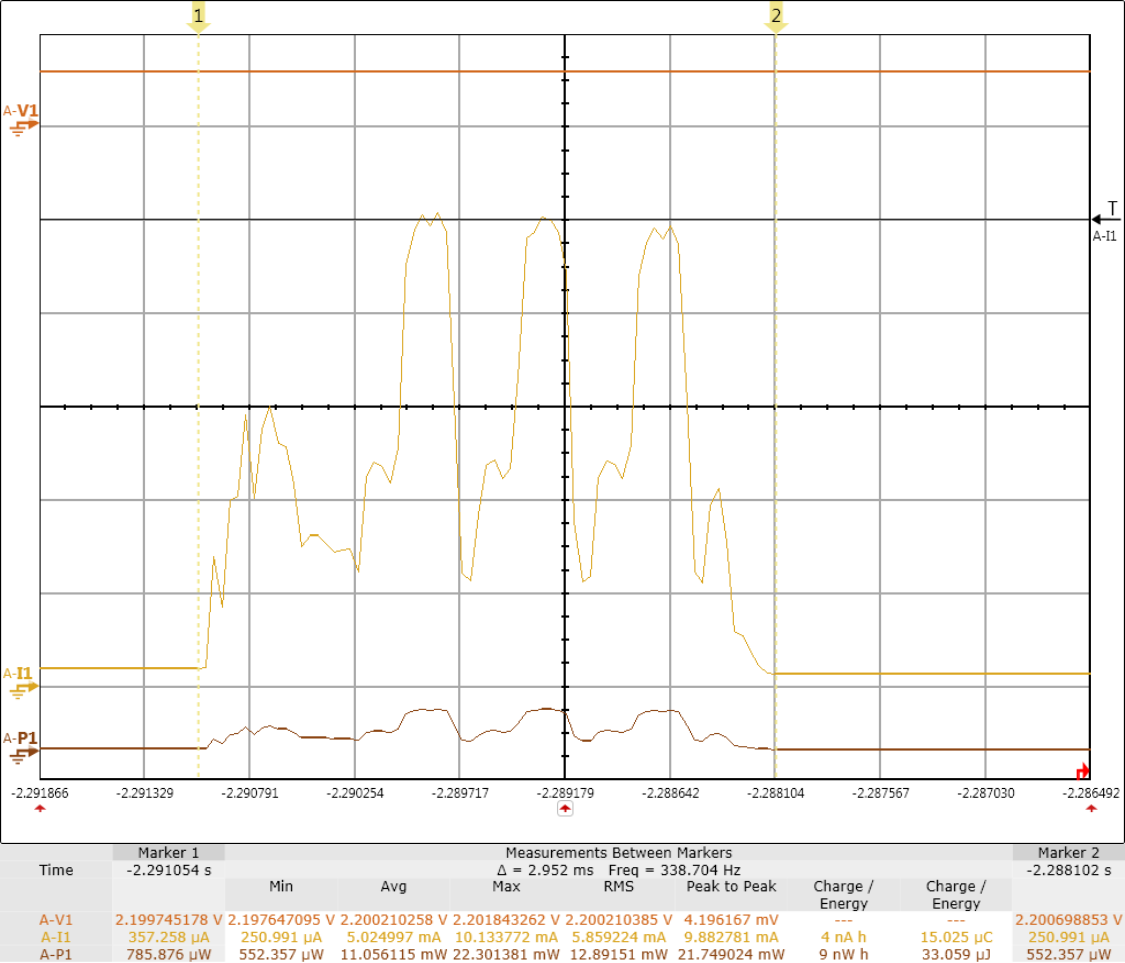
\includegraphics[scale=1]{3Vorgehen/imag/v0Send33uJ.png} 
    \caption{Minimalster Energieverbrauch: 3 BLE Pakte über Advertising Mode senden}
    \label{BLE_send}
\end{figure}

Um einen Anhaltspunkt über den Energieverbrauch des Sensortags zu erhalten, wurde 3 BLE-Pakete im Advertsing Mode per Knopfdruck gesendet (siehe Abbildung \ref{BLE_send}). Dies entspricht der Messung zur Sensortagversion V0. Nach der Weiterentwicklung des Programms, folgte die Messung V1, in der zusätzlich die GPIO ausgelesen werden. Dies ist für das Einlesen der Reed Switch-Impulse unumgänglich und für das Einlesen der Energy States vom 8500 sinnvoll. Die Version V2, erster Versuch mehr Sleep-Time einzubauen, scheiterete am Zusammenspiel des Timings der Radio- und GPIO-Interrupts. Das Neuaufsetzen des Programms half, sodass die Version V3 power-optimiert Geschwindigkeitspakete sendet. Die untenstehende Tabell stellt die ersten Energieresultate dar. Unterschieden wird zwischen dem Energieverbrauch für die Initialisierung und der Energie zum Senden von 3 BLE Paketen. Die Diskussion über Energieoptimierungen und die Deutung der Resultate finden sich in den Sitzungsprotokollen vom xxxxx - xxxx. Die Energiemessungen im Detail sind abgelegt auf der CD gemäss der Auflistung im Anhang xxxx.
\todo{Sitzungsprotokolle Datum einsezten, Anhanhgsbezeichnung}

\subsubsection*{Messresultate nach Sensortag-Versionen}
\begin{tabbing}
    Version   \quad\= Datum    \quad\= Was................................................... \quad\= Energie Init    \quad\=  Energie Senden \\[0.8ex]
    V0        \> 10.3.16  \> Nur BLE Paket      \> unbekannt            \> 33 $\mu$J \\
    V1        \> 16.3.16  \> mit Geschwindigkeit      \> 87 $\mu$J            \> 32 $\mu$J \\
    V3        \> 22.4.16   \> Schlafmodus optimiert     \> 40 $\mu$J            \> 29 $\mu$J \\
    V4        \> 03.6.16    \> 3 Sensore, kein Schlafmodus optimiert     \> 77 $\mu$J            \> 43 $\mu$J \\
\end{tabbing}

Bei den ersten drei Messungen werden die Sensoren noch nicht ausgelesen. Es zeigt sich, dass das Auslesen der Sensoren über I2C und das Warten, bis dass die Sensoren aufgestartet sind, viel mehr Energie verbraucht, als erwartet. Der Energieverbrauch des Auslesens nur eines Sensors (erste Priorität hat laut Aufgabenstellung der Drucksensor) ist ohne Optimierungsmassnahmen so gross, dass kein Senden der Daten mehr möglich ist. Die Speisung der Applikation bricht sofort zusammen (siehe Abbildung \ref{i2c_problem}).
\todo{warum ht sich BLE verschlechtert?}

\begin{figure}[ht]
    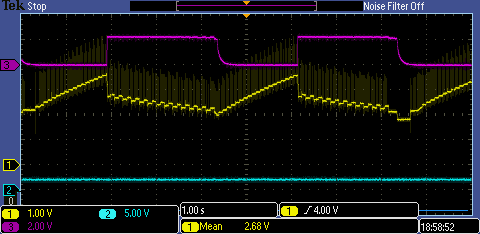
\includegraphics[scale=1]{3Vorgehen/imag/pic4VSUPbrichtEin.PNG} 
    \caption{Auslesen der Sensoren reisst Energie zusammen}
    \label{i2c_problem}
\end{figure}

\todo{Bild erscheint nicht}

Aus diesen Grund wurde die Power-Optimierung innerhalb des Programms zur zentralen Herausforderung in dieser Arbeit. Details darüber sind im nächsten Unterkapitel \ref{powerOptimierung} Power Management zusammengefasst. Hier die Auflistung der Energiewerte von Version V4. Bei dieser Version werden die Sensoren ausgelesen und dazwischen geht das Sensortag in den Schlafmodus, damit sich der Primärkondensator wieder laden kann. Erst nachdem alle Sensoren ausgelesen sind, wird das BLE-Paket versendet.



\subsubsection{Sensortag}
\label{energie senosortag} 

Der Energieverbrauch des Sensortags wird 4-mal gemessen. Einmal mit der Minimalversion: Nur Pakete mit Geschwindigkeitsdaten senden. Dann diese Version mit den drei Sensoren, die einer nach dem anderen ausgelesen werden. Weil dazwischen geschlafen wird, damit das System wieder genug Energie gespeichert hat, dauert diese Version xxx s \todo{Zeit eintragen}. Von jedem Sensor wird der eigene Energieverbrauch ermittelt, um einen Vergleich unter ihnen herstellen zu können.

\paragraph{Nur Geschwindigkeit: Simple Harvester}

\todo{Energiemesssung OHNE Sensoren. Aber mit Warten}

%\begin{figure}
%  
\includegraphics[width=1.0\textwidth]{idle.png}
%  \caption{Energieverbrauch nur Geschwindigkeit Senden V4}
%  \label{messung_v}
%\end{figure}



\paragraph{Energieverbrauch Drucksensor}

Auf dem Sensortag wird der Drucksensor BMP 208 von Bosch Sensortec verwendet. Der Druckwert wird über I2C ausgelesen. Hier die Energiemessung des Sensors, ausgelesen mit der Sensortag Version 4, am 3. Juni 2016.

\begin{figure}[ht]
  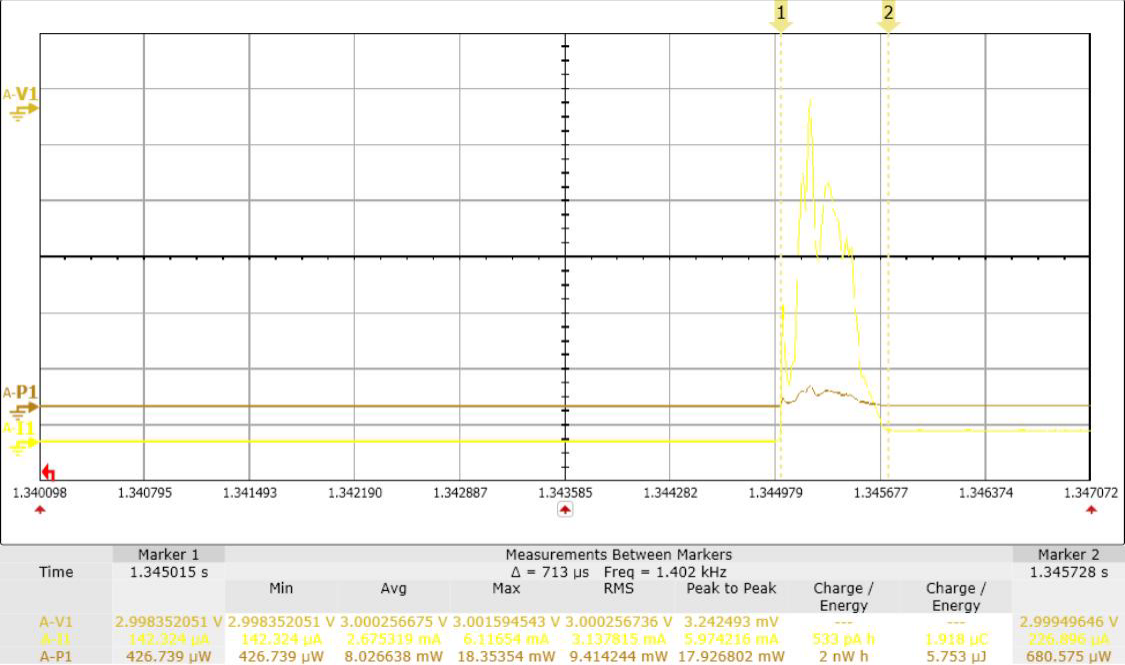
\includegraphics[width=1.0\textwidth]{3Vorgehen/imag/Drucksensor.png}
  \caption{Energieverbrauch des Drucksensors BMP 280}
  \label{energie_drucksensor}
\end{figure}

Das Auslesen des Drucksensors verbraucht 5.753 $\mu$J.

\paragraph{Energieverbrauch Temperatursensor}

\todo{tempsensor daten}
Der Temperatursensor xxx der Marke yyy verbraucht fürs Auslesen der Daten, ohne Energieoptimierung, 10.635 $\mu$J.

\begin{figure}[ht]
  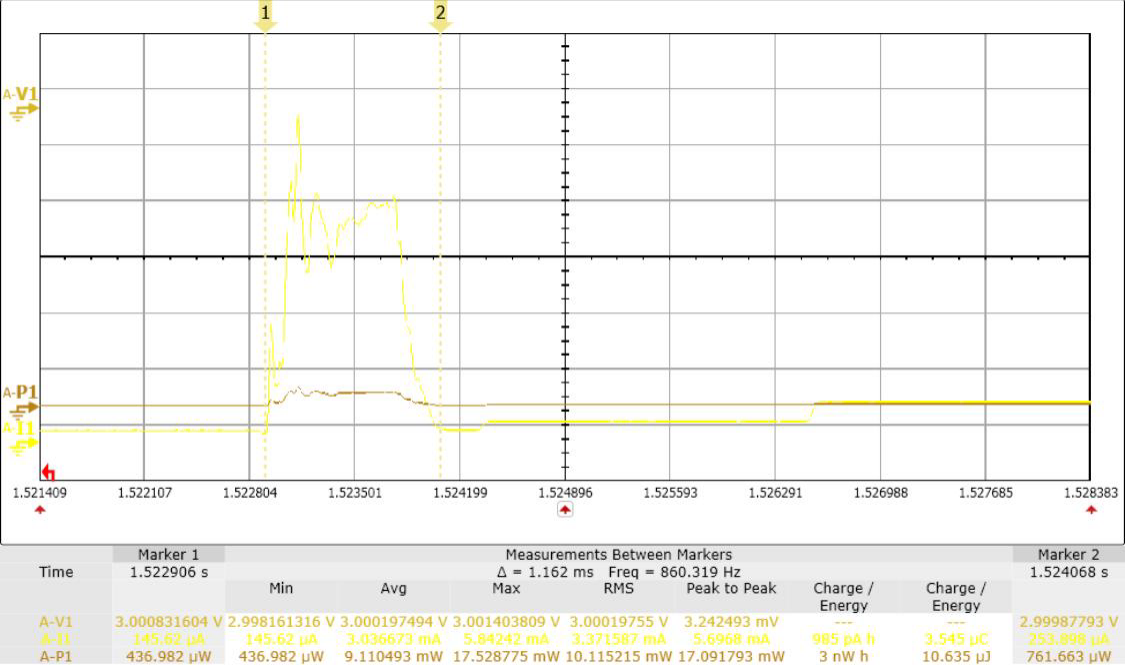
\includegraphics[width=1.0\textwidth]{3Vorgehen/imag/tempSensor.png}
  \caption{Energiemessung Temperatursensor auf Sensortag}
  \label{energie_tempsensor}
\end{figure}


\paragraph{Energieverbrauch Feuchtigkeitssensor}

Der Feuchtigkeitssensor verbraucht 6.358 $\mu$J, siehe Abbildung \ref{energie_humidity}.

\begin{figure}
  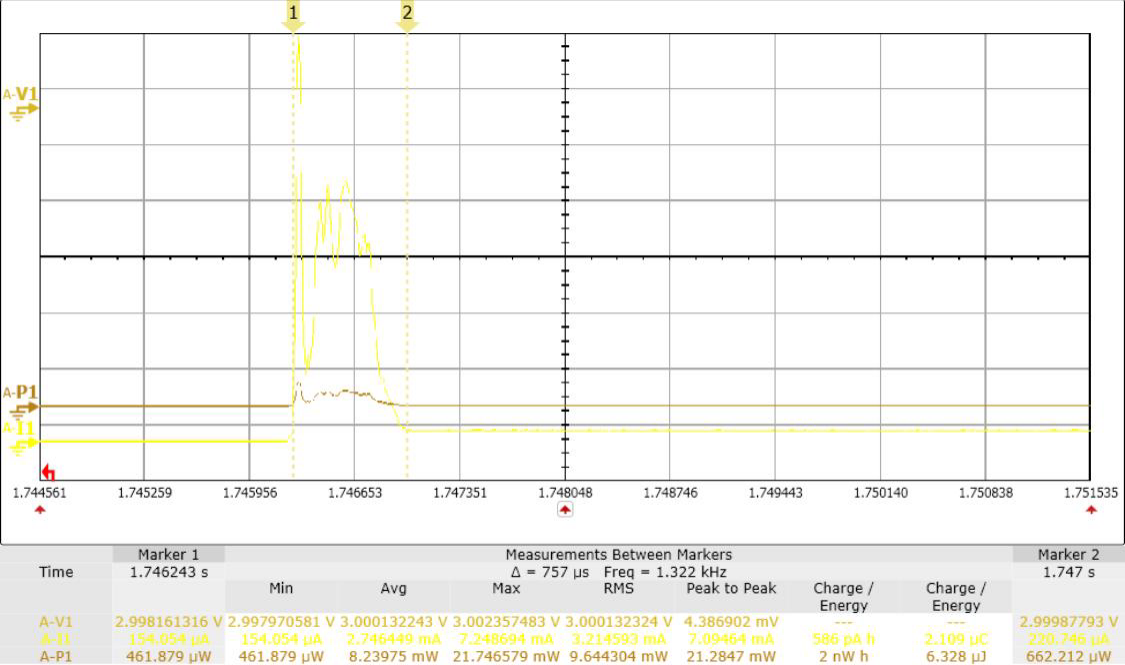
\includegraphics[width=1.0\textwidth]{3Vorgehen/imag/Humidity.png}
  \caption{Energieverbrauch Feuchtigkeitssensor}
  \label{energie_humidity}
\end{figure}




% x.2 ---------------------------------
\subsection{Energiekalkulation}
\label{v_e_kalkulation}

Der Energieverbrauch hängt von der Anzahl ausgelesener Sensoren ab (siehe \ref{v_messungen_sensortag}). Für die Bestückung der Kondensatoren wird vom schlechtesten  Fall, einer Geschwindigkeit von 10 km/h ausgegangen. Die Grundlagen zur Energiekalkulation $\bar{E_{HRV}} \ge \bar{E_{BLE}} $ sind im Theorieteil \ref{th_energiebilanz} abgebildet. Hier werden die Kondensatoren berechnet.

\todo{Gleichungen zusammen. Berechnung konkret}
\begin{equation}
  C_{STS}= \frac{ E_{Applikation}}{(V_{STS\_HIGH} )^2 - (V_{STS\_LOW} )^2}
\end{equation}

\begin{equation}
  C_{STS}= \frac{ E_{Applikation}}{(3.6 V )^2 - (2.1 V)^2}
\end{equation}

\begin{equation}
  C_{STS}= \frac{ E_{Applikation}}{(3.6 V )^2 - (2.1 V)^2}
\end{equation}

\begin{equation}
  C_{STS}= \frac{ E_{Applikation}}{(3.6 V )^2 - (2.1 V)^2}
\end{equation}


\todo{Abschlusstext. Übergang}

\subsubsection{MPP einstellen}

\todo{Messprotokolle eintrage}

Das Ziel der Entwicklung ist, dass bei einer Geschwindigkeit von 10 km/h genug Enerige zum Senden eines BLE-Pakets zur Verfügung steht. Während der Entwicklung des Harvesters wurde die Leistungskurve öfters aufgenommen (siehe Anhang \ref{uebersicht_messprotokolle}, xxx,yyy, zz). Wie im Theorieteil erklärt \ref{harv_diff} unterscheidet sich das Leistungsmaximum nach Geschwindigkeit. Weil das Ziel ein funktionstüchtiger Prototyp bei 10 km/h ist, bezieht sich das Einstellen nur auf diese Wert.  

 
\subsubsection*{MPP-Ratio bei 10 km/h gemäss Messprotokollen}
\begin{tabbing}
    Datum       \quad\= Leistungmaximum    \quad\= MPP-Ratio\\[0.8ex]
    30. März    \> 12 $\mu$W        \> 43.23\thinspace\% \\
    xx          \> xx $\mu$W        \> xx\thinspace\%\\
    resultat    \> 21.87  $\mu$W    \> 24.87\thinspace\%\\
\end{tabbing}\todo{Werte}

Es zeigt sich, dass das Leistungsmaximum unterhalb von 50\thinspace\% liegt. Bedauerlich ist, dass durch die Energieoptimierung sich die Stelle des Leistungsmaximums Richtung Leerlauf verschiebt. In der Umsetzung mit dem EM8500-Chip ergibt sich das Problem, dass nur Konfigurationen von MPPT-Ratios von 50 - 80\thinspace\% erlaubt sind (siehe Tabelle unten).  Die Einstellungen der tieferen MPP-Ratio sind zudem gröber. Dies, weil der EM8500-Chip für Harvester vom Typ TEG (mit einem MPP konstant bei 50\thinspace\%) und Solarzelle konzipiert ist und die MPPT-Ratio für diese zwei Anwendungen genau in diesem Range liegen. In unserem Fall ist dieser vorgegebene Range nicht ideal. Da beim energiekritischen Zustand bei 10 km/h die Ratio deutlich unter 50\thinspace\%. Die Vorgänger wählten in ihren Einstellungen eine MPPT-Ratio von 88\thinspace\%. Die Vermutung liegt nahe, dass keine Leistungskurve des Harvesters im Voraus aufgenommen wurde.


\subsubsection*{MPPT-Ratio Einstellungen EM8500}
\begin{tabbing}
    Registerwert   \quad\= MPPT-Ratio    \\[0.8ex]
    0x00           \> 50\thinspace\% \\
    0x01           \> 60\thinspace\%\\
    0x02           \> 67\thinspace\%\\
    0x03           \> 71\thinspace\%\\
    0x04           \> 75\thinspace\%\\
    0x05           \> 78\thinspace\%\\
    0x06           \> 80\thinspace\% \\
    0x07           \> 82\thinspace\%\\
    0x08           \> 83\thinspace\%\\
    0x09           \> 85\thinspace\%\\
    0x0A           \> 86\thinspace\% \\
    0x0B           \> 87\thinspace\%\\
    0x0C           \> 88\thinspace\%\\
\end{tabbing}

\todo{Sitzungsprotokoll Datum}
Im ersten Versucht wird das Register auf das Minimum (50\thinspace\%) eingestellt (siehe Sitzungsprotokoll YYYY). Die Messung ergab, dass bei 10 km/h das EM-Board nicht gespiesen wird. So luden sich weder der STS noch der LTS auf. Der Grund ist, dass der optimale Leistungsbezug bei 50\thinspace\% liegt, das Leistungsmaximum aber später. So entstand beim Regeln auf den optimalen Leistungsbezug der Umstand, dass dort nur 0.2 V produziert werden. Dieser Spannungswert ist zu tief, der EM-Chip beginnt nicht zu arbeiten. Betreibt man den Harvester nicht am optimalen Punkt, sondern bei einer MPPT-Ratio von 60\thinspace\%, so wird eine Eingangsspannung von 0.3 V produziert und EM8500 beginnt zu arbeiten.




% x.3 -------------------------------------
\subsection{Einstellen der Schwellwerte}
\label{v_schwellwerte}

Das Konzept der Schwellwerte von VSTS und VLTS sind im Theorieteil bei der Erklärung des Speicherkonzepts des EM8500-Chips im Unterkapitel \ref{speicher_konzept} beschrieben. Das Ziel ist, dass bei 10 km/h sich LTS entlädt. Die Berechnung der Schwellwerte stammt aus dem Theorieteil \ref{th_energiebilanz}.




Aus der Vorgängerarbeit sind in der Tabelle unten notierte Konfigurationswerte überliefert. Bei der Inbetriebnahme fiel der hohe Schwellwert von v\_bat\_min\_hi\_dis auf (3.6 V), ab der erst die Applikation gespiesen wird. Den hohen Wert beruht auf dem Versuch, möglichst viel Energie vor dem Datensenden zu sammeln. Ein hoher Schnellwert verzögert die Zeit, bis zum ersten Datensenden.

\subsubsection*{Konfiguration Vorgängermodell}
\begin{tabbing}
    Register .............\quad\= Wert \\[0.8ex]
    v\_bat\_max\_hi       \> 4.2 V \\
    v\_bat\_max\_lo       \> 4.1 V \\
    v\_bat\_min\_hi\_dis  \> 3.6 V \\
    v\_bat\_min\_hi\_con  \> 2.1 V \\
    v\_bat\_min\_lo       \> 1.8 V \\
    v\_appl\_max\_hi      \> 3.8 V \\\
    v\_appl\_max\_lo      \> 3.7 V \\ 
    mppt\_ratio            \> 88\thinspace\% \\
\end{tabbing}

Nach der Energiemessungen der Version V3 des Sensortags (siehe \ref{erst_EMessungen}), in dem die Geschwindigkeit per BLE gesendet werden kann, entstanden folgende Schwellwerte:

\subsubsection*{Erste Konfiguration aufgrund Geschwindigkeitsmessung}
\begin{tabbing}
    Register .............\quad\= Wert \\[0.8ex]
    v\_bat\_max\_hi       \> 4.8 V \\
    v\_bat\_max\_lo       \> 4.7 V \\
    v\_bat\_min\_hi\_dis  \> 2.6 V (siehe Berechnungen unten)\\
    v\_bat\_min\_hi\_con  \> 2.1 V \\
    v\_bat\_min\_lo       \> 2.0 V (vorgegeben von Sensortag)\\
    v\_appl\_max\_hi      \> 3.8 V \\\
    v\_appl\_max\_lo      \> 3.7 V \\ 
    mppt\_ratio            \> 50\thinspace\% (aus MPP-Kurve Harvester)\\
\end{tabbing}

Die Grundlage bildete die Gleichung  $E_{Applikation}= E_{STS\_HIGH} - E_{STS\_LOW}$, wobei  $E_{Applikation}$ aus der Messung von V3 mit total 93.2 $\mu$J für die Initialisierung und das Senden der Daten gebraucht werden, und $V_SUP$ durch das Sensortag mit 2.0 vorgegeben ist. Laut Datenblatt des EM8500 (\cite{datasheet_EM85}, S. 9, Abschnitt Operating Conditions ) soll STS zwischen 10 - 100 $\mu$F gross sein. Typisch ist 47 $\mu$F. Um auf der sicheren Seite zu sein, denn der Harvester gibt zu diesem Zeitpunkt noch nicht genug Energie ab, wurde als Berechnungsgrundlage C\_{STS} von 100 $\mu$F genommen.  So ergab sich folgender minimaler oberere Schwellwert:

\begin{equation}
(v\_bat\_min\_low) ^2  =  \frac{2\, \times \, E_{Applikation}}{C_{STS}} + (V_{STS\_LOW})^2
\end{equation}

\begin{equation}
(v\_bat\_min\_low) ^2  =  \frac{2\, \times \, 93.2, \mu J}{100 \,\mu F} + (2.0)^2
\end{equation}

\begin{equation}
v\_bat\_min\_low  =  \sqrt{\frac{186.4}{100 } + 4} = \sqrt{5.864} = 2.42 V
\end{equation}

Alternativ kann man den laut Datenblatt vorgeschlagenen Kondensatorenwert von  47 $\mu$F. Dann ergibt sich als oberer Schwellwert  $v\_bat\_min\_low  =  \sqrt{\frac{186.4}{47 } + 4} = \sqrt{7.97} = 2.82, V$. Als erstes wird der Schwellwert auf 2.6 V gesetzt. Wichtigster Wert in der Konfiguration ist jedoch der korrekte MPPT-Wert. Er wird auf das Minimum (50\thinspace\%) gesetzt. Das Maximum des Ladezustands  wird auf den maximal erlaubten Wert gesetzt: v\_bat\_max  = 4.8 V bzw. 4.7 V. Denn solang Energie geerntet werden kann, soll sie gespeichert werden. v\_appl\_max spielt in unserer Anwendung keine wichtige Rolle. Der Wert wird von den Vorgängern übernommen.

\todo{Messprotokoll und Sitzungsprotokoll einfügen}
Das Zusammensetzen der Last (Sensortag) mit der konfigurierten Hardware erstaunte (siehe Messprotokoll xxx und Sitzungsprotokoll yyy). Ab 25 km/h funktionierte die Schaltung gut. Doch darunter reagiert der EM8500-Chip nicht. Weder STS noch LTS konnten sich laden. Nachmessungen am Eingang vom EM8500-Chip ergaben, dass bei  10 km/h und einer MPPT-Ratio von 50\thinspace\% eine Spannung von 0.2 V anliegt. Diese ist zu tief, um den Booster zu starten. Erst bei höherer Geschwindigkeit wird eine Eingangsspannung von mehr als 0.3 V erreicht, und das System beginnt zu funktionieren. Aus diesem Grund wird die MPPT-Ratio zukünftig auf den zweittiefsten Wert (60 \thinspace\%) eingestellt. 

Ein unerwartetes Verhalten zeigt sich bei der Implementation des Auslesen des ersten Sensors, der Drucksensor. Der BLE-Sniffer empfängt die Druckdaten korrekt, doch beim Anschliessen des Sensortags an den Harvester, riss die Spannung sofort zusammen. Innert kürzester Zeit haben sich entlädt sich der STS wie parallel zu ihm der LTS und unterschreitet der STS den Schwellwert von V\_SUP von 2 V, so stellt die Speisung der Applikation ab (siehe Abbildung \ref{i2c_problem} im Unterkapitel \ref{erst_EMessungen}). Das Ausmessen des Energieverbrauchs bringt Klarheit: Die I2C-Kommunikation und das Aufstarten des Sensors brauchen xxx-mal mehr Energie, als das Berechnen der Geschwindigkeit aus den Reed-Switch Impulsen (siehe Abbidlung yyy im Resultat-Teil).
\todo{link zu Abbildung im Resultat Teil. Faktor ausrechnen}

Durch den deutlich höheren Energieverbrauch, wird eine Power-Optimierung im Softwareteil notwendig. Es zwingt aber auch, den Schwellwert von v\_bat\_min\_hi\_dis  wieder zu erhöhen. Die finale Konfiguration ist im Resultate-Teil abgebildet.


% x.4 -----------------------------------------
\subsection{Energiezustand des Systems}
\label{v_energiezustand}

Die letzte der vier Aufgaben aus der Optimierungsliste nach der Inbetriebnahme (siehe Unterkapitel \ref{optimierung}) ist das variable Anpassen des BLE-Paketsendens aufgrund des Energiezustandes. Im ersten Unterkapitel \ref{def_zustaende} wird das Einteilen des Systems in Energiezustände beschrieben, danach die Umsetzung in Software im Prototyp angewendet wurde. 

\subsubsection{Definition von Energiezuständen}
\label{def_zustaende} 

\
Da die produzierter Energie von der Fahrgeschwindigkeit abhängt, wird das Energiesystem in drei Zustände eingeteilt, die von der Geschwindigkeit abhängen:

\subsubsection*{Energiezustände aufgrund der Geschwindigkeit}
\begin{tabbing}
   0 - 15 km/h      \quad\= LOW\_ENERGY   \\[0.8ex]
   15 - 25 km/h      \> MIDDLE\_ENERGY \\
   $>$ als 25 km/h   \> HIGH\_ENERGY\\
    
\end{tabbing}

Was in den eingelnen Energiezuständen gemacht wird:

Bild

\subsubsection*{Energiezustände: Umsetzung in Software}






 4---------------------------------------------------------------------------
\section{Power Management}
\label{powerOptimierung}

Aufgrund von Messungen -> Codeoptimierung


%... noch zu schreiben ....
%Üblicherweise wird das RTOS-Betriebssystem von TI für Low Power Applikationen benutzt. 


%(Die Low-Power Programmbeispiele von TI basieren auf RTOS, ebenso die Dokumentation zu Low Power Applikationen, was zu viel Energie verbraucht (korrekt, wie belegen?). )


%Problem: So gehört zu jedem Aufwecken einer Peripherie, der Parallele Schlafmodus, bis dass die Peripherie gestartet ist. (Dies gilt auch für die Sensoren.) Zu lange warten: braucht Energie.
%
%Sleep konkret: Power Banks abschalten:\\
%Power Domains zeigen
%
%Schwierigkeit Interrupt and Events !!
%
%Bild: Energie-Langzeitmessung BLE versenden\\
%Beschriften mit aktiv und standby modus
%
%
%Gearbeitet wird mit einem Cortex M3 von TI.\\ 
%Grundsätzlich basieren die Bsp. auf RTOS. Wenige für PowerManagement. Das Powermanagement ohne Betriessystem. Wir verwenden dies, weil (gemäss Erfahrungswerte Praxis) mit Betriebsystem mehr Energie braucht).


\begin{figure}
  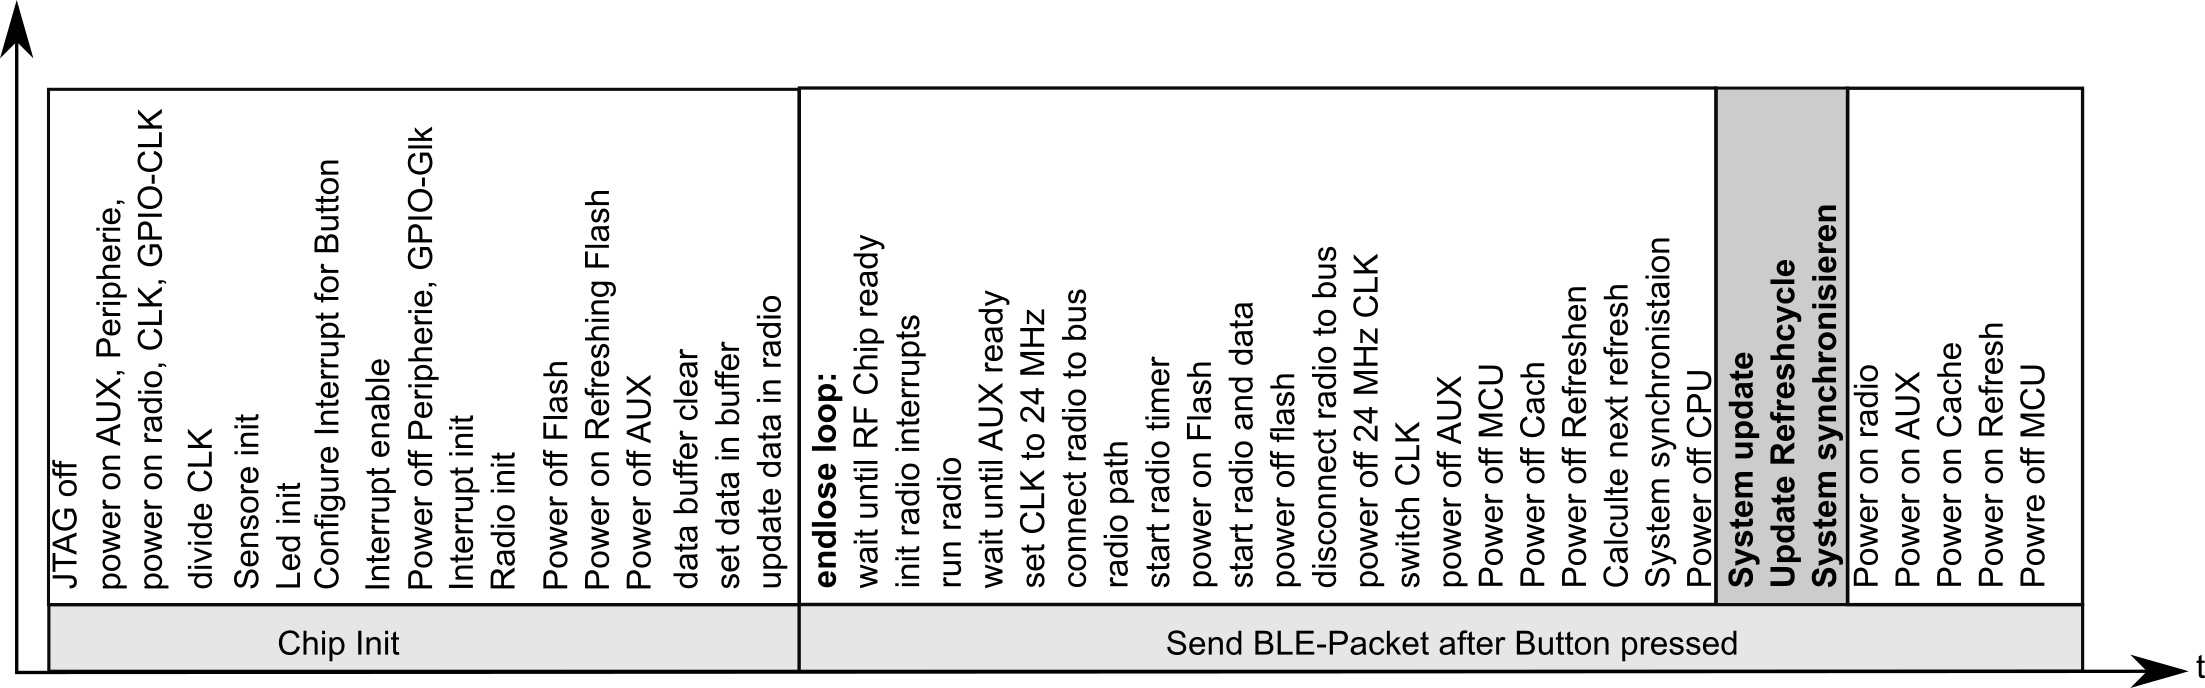
\includegraphics[width=1.0\textwidth]{../ressources/SimpleLink/V0Sendeablauf.png}
  \caption{Prozessablauf V0}
\end{figure}




% 5 ---------------------------------------------------------------------------
\section{Applikationsentwicklung}
Nachfolgend wird der Aufbau von TI SensorTag zusammen mit unserem selbst entwickelten Board als Sensor benannt und die Android Applikation auf dem Smartphone wird einfach als Applikation benannt.
\subsection{Aufbau der Applikation}
\begin{figure}
    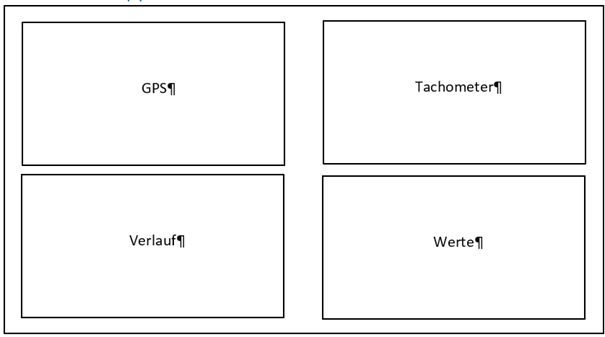
\includegraphics{3Vorgehen/imag/Aufbau_Applikation_erste_Version.PNG}
    \caption{Aufteilung des Bildschirms}\label{aufbau_applikation_1} 
\end{figure}
Der Aufbau der Applikation soll Anfangs in vier Teile des Bildschirms geteilt werden. 
Im Bereich GPS soll eine Karte angezeigt werden, ausserdem soll es möglich sein die Route aufzuzeichnen und abzuspeichern.
Der Verlauf zeigt die Entwicklung der Geschwindigkeit über einen gewissen Zeitraum, wobei es wählbar sein soll welche Daten angezeigt werden.
Die Geschwindigkeit soll anschaulich in einem Tachometer angezeigt werden und die Tachonadel soll im besten Fall animiert sein.
Im Bereich der Werte sollen die aktuellen Werte in Zahlen und den entsprechenden Einheiten dargestellt werden.
Schnell wurde klar, dass dieser Aufbau wenig Sinn macht, da die Bereiche auf einem Smartphone viel zu klein wären und nicht mehr leserlich sein würden. Darum wurde ein neues Konzept erarbeitet, welches in der Abbildung x ersichtlich ist.

\subsubsection{Home-Screen}
Als erstes soll der Benutzer den sogenannten Home-Screen sehen, hier werden der Tachometer, die Werte und ein paar Buttons angezeigt. Je nach Anzahl der Funktionen sollen neue Buttons implementiert werden. So soll beispielsweise für die Sensorwahl ein Button vorhanden sein. Während der Entwicklung der Applikation wurde die Idee von einer GPS-Karte und einem Verlauf ebenfalls verworfen, da diese Funktionen aus zeitlichen Gründen nicht mehr realisierbar waren. Jedoch wäre der Home-Screen in der Lage mehr Buttons aufzunehmen, es muss nur darauf geachtet werden, dass die Anzeige der Werte nicht zu gross wird.

\subsubsection{Sensorwahl}
Schnell wurde klar, dass die Auswahl eines spezifischen Sensors wichtig werden würde, für den Fall, dass einmal mehrere Sensoren vorhanden wären. Ein Beispiel, würde unsere Applikation bei einem Fahrradrennen eingesetzt werden, so müsste die Applikation auf dem Smartphone mit dem Sensor am Fahrrad gepaart werden. Ansonsten würde man die Daten von allen Sensoren empfangen und die Anzeige würde nicht die Daten des eigenen Sensors anzeigen.

\subsubsection{Einheiten und Einstellungen}
Es kam ebenfalls der Wunsch auf, die Einheiten der Werte, einstellbar zu machen, da die Applikation bestenfalls auch in anderen Ländern verwendet werden soll. Also wäre es optimal, wenn die Geschwindigkeit beispielsweise auch in Miles per Hour dargestellt werden könnte. Vielleicht müsste auch eine Einstellungsmöglichkeit bereitgestellt werden, damit die Temperatur kalibriert werden kann.

\subsubsection{BLE-Kommunikation}
Der wichtigste Teil der Applikation ist die Bluetooth-Kommunikation, hier werden die Daten vom Sensor empfangen. Die Daten müssen nach dem Empfangen gefiltert werden, damit sichergestellt wird, das die empfangenen Daten von einem unserer Sensoren kommen. Sobald sichergestellt ist, das die empfangenen Daten zu unserem Sensor gehört, müssen diese umgerechnet werden.

\subsubsection{Inbetriebnahme des Codes der PA}
Als erster Schritt wurde der Code der vorangegangenen Arbeit analysiert und die wichtigen Teile zur Bluetoothkommunikation übernommen. Es wurden folgende Funktionen aus dem Code übernommen: onStart, onActivityResult, scanLeDevice, BluetoothAdapter.LeScanCallback.

Die Funktion onStart wurde in BLE_init umbenannt und der Mechanismus zum Wachhalten des Geräts wurde entfernt. Der Mechanismus wurde entfernt, da dieser nicht mehr funktionierte. Ebenfalls wurde die Funktion in die Funktion onCreate eingefügt, um den Code übersichtlicher zu gestalten und da diese Funktion nur einmalig aufgerufen werden musste.
 
Die Methoden onActivityResult und scanLeDevice wurden komplett übernommen.

Die Callback-Funktion des Bluetoothadapters BluetoothAdapter.LeScanCallback wurde strukturell übernommen, jedoch wurde die Codierung zur Verarbeitung der Daten entfernt.

\subsubsection{Filter einbauen}
Der nächste logische Schritt war, dass die empfangenen Daten gefiltert werden mussten. Dafür wurde folgende Struktur definiert, damit festgestellt werden kann, ob die Daten von einem unserer Sensoren versendet wurden.
\begin{tabbing}
   Length	\quad\= Type	\quad\= UUID 	\quad\= Package ID	\quad\= Speed	\quad\= Pressure	\quad\= Temperature	\quad\= Humidity	\quad\= Checksum   \\[0.8ex]
   23	\> 0x03	\> 0xDEBA \> 2 bytes\> 4 bytes\> 4 bytes\> 4 bytes\> 2 bytes \\
\end{tabbing}
Aufgrund dieser Struktur können alle empfangenen Daten, welche nicht die definierte Länge, Typ und UUID besitzen, ignoriert werden.

Wenn sichergestellt ist, dass die Daten von unserem Sensor stammen, musste noch die Adresse vom Sender gespeichert werden. Alle Adressen werden in einer Liste gespeichert, vor dem Speichern wird jedoch noch geprüft, ob die Adresse bereits in der Liste ist, falls ja wird die Adresse nicht noch einmal gespeichert.

\subsubsection{Berechnung der Daten}
Der Sensor sendet Werte, wie den Zeitunterschied zwischen zwei Magnetdurchläufen, dem Luftdruck, der Temperatur und die relative Luftfeuchtigkeit. Diese Daten müssen erst noch in die realen Werte umgerechnet werden, da alle Werte in mehreren Bytes verteilt vorliegen.

Der Zeitunterschied zwischen zwei Magnetdurchläufen wird in vier Bytes dargestellt. Die ersten beiden Bytes enthalten die Anzahl Sekunden, es muss also das erste Byte um acht Bit geschoben werden und anschliessen muss das zweite Byte noch addiert werden. Folgende Formel zeigt die Umrechnung von zwei Bytewerten in eine reelle Zahl:
\todo{Formel einfügen}
Die erhaltene Zahl muss noch mit einem Typecast in den Datentyp float umgewandelt werden.

Das dritte und vierte Byte des übermittelten Zeitunterschieds enthält die Sekundenbruchteile. Folgende Formel zeigt, wie die Bytes verrechnet werden müssen, um die korrekten Werte zu erhalten:
\todo{Formel einfügen}
Der erhaltene Sekundenbruchteil kann nun zu den ganzen Sekunden dazu addiert werden, um die ganze Zeit zwischen zwei Magnetdurchläufen zu erhalten.

Ein Beispiel, wird also der hexadezimale Wert 0x00014000 empfangen sind das 1.25 Sekunden zwischen zwei Magnetdurchläufen.

Um die Geschwindigkeit zu erhalten muss der Radumfang durch die erhaltene Zeit geteilt werden. Jedoch befinden sich an unserem Rad zwei Magnete, deswegen darf nur der halbe Radumfang verrechnet werden. Ausserdem ist das Resultat in m/s und muss deshalb noch in km/h umgerechnet werden, was nichts anderes als eine Multiplikation mit dem Faktor 3.6 ist.

Der Druck wird in Pa übertragen, hier müssen die verschiedenen Bytes miteinander addiert werden und in hPa umgerechnet werden. Es werden jedoch nur die letzten drei Bytes mit Werten befüllt sein, das erste Byte kann ignoriert werden. Folgende Formel zeigt die Umrechnung der Bytes in eine float Zahl.
\todo{Formel einfügen}



\subsection{Grundeinstellungen}

\subsection{Tachometer einbauen}

\subsection{Modularer Aufbau}

Die Applikationsentwicklung basiet auf einer modularen Struktur.  Dadurch wird eine Weiterentwicklung der Applikation ohne Probleme möglich. Ebenfalls wurde beachtet, dass die Applikation sogar in andere Sprachen übersetzt werden können muss, dafür wurden alle Texte, die ersichtlich sind in einem File aufgenommen und können zentral abgeändert werden, ohne einen Eingriff in den aktuellen Code.


Mit Android Version xx.

--- alter Text --- 

\subsection{Aufbau der App}

Welche Aktion zu welchem Display gehört (Überblick Gesamtsystem)


\subsection{Implementierte Aktionen}
Geräteauswahl
Kalibrierung
Geschwindigkeitsberechnung
Sensordaten ausgeben (was mit welcher Genauigkeit)

\subsection{BLE Empfangen}

Aufbau des Datenpakets: 
LEN, UUID, ...






